% !TeX root = ../praktikum.tex
% !TeX encoding = UTF-8
% !Tex spellcheck = de_DE


Anhand der aufgenommenen Messdaten des Versuchsteils zur Winkelabhängigkeit wurde nun die Abhängigkeit des Quanten-Hall-Effekts, sowie des Shubnikov-de Haas-Effekts vom Einfallswinkel des Magnetfeldes auf die Probe analysiert.
Dazu wurden in Abbildung %TODO: GRAPH 
die Magnetfeldwerte der Minima in Abhängigkeit des Winkels zur Probennormalen aufgetragen. 
In der Graphik ist gut zu erkennen, dass die Shubnikov-de Haas-Oszillationen, sowie die Quanten-Hall-Plateaus innerhalb eines Winkels von $110^\circ$
noch recht gut zu erkennen sind und ab einer Auslenkung von $120^\circ$
aus der senkrechten Position der Probe zu den Magnetfeldlinien verschwinden. Erklärt werden kann diese Beobachtung mit der Tatsache, dass ab dieser Auslenkung keine Hallspannung mehr über die Breite der Probe induziert wird, die Voraussetzung selbst für den klassischen Halleffekt nicht mehr erfüllt ist.  %TODO: fällt dir hier ne schönere Formulierung ein?: Eine geringe Auslenkung der Probenebene aus den idealerweise senkrechten eintreffenden Magnetfeldlinien, führt zu einer Abschwächung des Effekts, bis der Winkel zu steil wird und die Magnetfeldlinien keine Hallspannung mehr induzieren können...?


\begin{figure}[h]
	\centering
	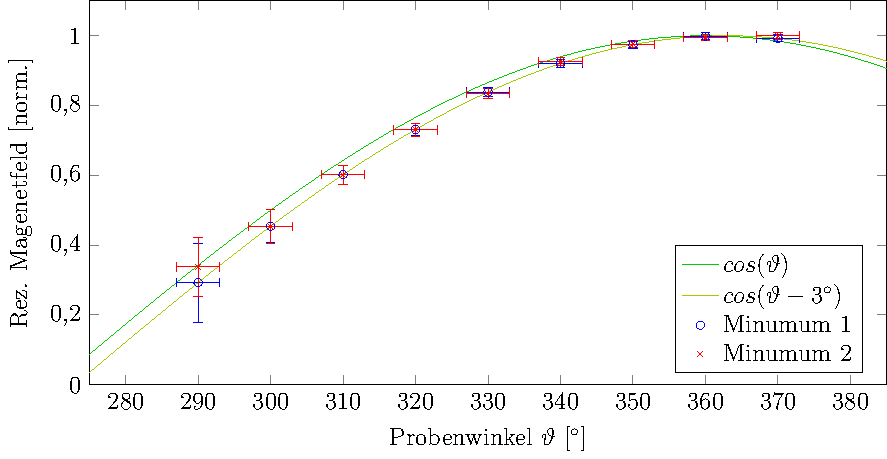
\includegraphics[scale=1]{graphs/winkel/auswertung.pdf}
	\caption[]{
		}
		\label{fig:winkel_ausw}
\end{figure}

